\documentclass[a4paper,twoside]{article}

\usepackage{epsfig}
\usepackage{subcaption}
\usepackage{calc}
\usepackage{amssymb}
\usepackage{amstext}
\usepackage{amsmath}
\usepackage{amsthm}
\usepackage{multicol}
\usepackage{pslatex}
\usepackage{algorithm2e}
\usepackage[bottom]{footmisc}
% Please add other packages that you may need BEFORE the SCITEPRESS.sty package.
\usepackage{natbib}
\usepackage{multirow}
\usepackage{SCITEPRESS}

\begin{document}

\title{Analysis of Programming Students' Prompts to Identify Interactions
Patterns with Generative AI}

\author{\authorname{Rodrigo Prestes Machado\sup{1}\orcidAuthor{0000-0003-0428-6387},
Carlos Alario Hoyos\sup{2}\orcidAuthor{0000-0002-3082-0814} and
Carlos Delgado Kloos\sup{2}\orcidAuthor{0000-0003-4093-3705}}
\affiliation{\sup{1}Department of Informatics, Federal Institute of Education,
Science and Technology, Porto Alegre, Brazil}
\affiliation{\sup{2}Department Telematics Engineering, Carlos III University,
Madrid, Spain}
\email{\ rodrigo.prestes@poa.ifrs.edu.br, \{calario,cdk\}@it.uc3m.es}
}

\keywords{Generative Artificial Intelligence, Programming Education, Chatbots}

\abstract{The abstract should summarize the contents of the paper and should
contain at least 70 and at most 200 words. The text must be set to 9-point font
size.}

\twocolumn\maketitle\normalsize\setcounter{footnote}{0}

\section{\uppercase{Introduction}}
\label{sec:introduction}

%What is the problem to be solved?

Recent advancements in Generative Artificial Intelligence (GenAI) have opened
up new possibilities in education. In programming courses, students can utilize
GenAI tools to improve their understanding, receiving assistance, feedback, and
detailed explanations.

The study of \cite{chan23} revealed that both undergraduate and postgraduate
students exhibit positive attitudes toward the use of GenAI in teaching and
learning, noting that it enhances the depth of their thinking and understanding.
Additionally, a systematic review conducted by \cite{Lo24} demonstrated that
students could effectively learn from ChatGPT, leading to improved understanding
and academic achievement. Besides of that, it was also observed that ChatGPT
enables students to regulate their learning pace, promoting self-regulation
\citep{Baha24} \citep{cai23}.

In the other hand, researchers have concerns about the impact of these
tools on students. The systematic review of \cite{Murillo23} indicated that
ChatGPT use might lead to an overreliance on the tool. \cite{chan23} also noted
that this reliance could result in a decrease in critical thinking, as students
might make decisions based solely on the information provided by ChatGPT.

The student's confidence is warranted, as shown by \cite{Puryear22}, who
demonstrated that GitHub Copilot can generate solutions for student assignments
with accuracy rates ranging from 68\% to 95\%. However, this raises concerns that
students might rely too heavily on GenAI tools, potentially neglecting a deeper
understanding of the underlying concepts. \cite{cai23} further identified
overdependence and reduced intellectual engagement as significant drawbacks of
using ChatGPT in learning.

Regardless of teachers' preferences or beliefs, preliminary surveys
performed by \cite{Dickey24} revealed that at least 54.5\% of students are
already using GenAI for homework. This highlights the need to understand how
students are interacting with these tools and how they can be used to enhance
learning. Furthermore, a review by \cite{Lo24} emphasized the necessity for
extended studies and objective measures to gather more robust evidence on the
use of GenAI tools in education.

% Are there any existing solutions?

To deal with this issue, some researchers have proposed different pedagogical
strategies \cite{Denny24} introduced the concept of \textit{Prompt
Problems}, where students solve programming exercises by formulating natural
language prompts. \cite{Prasad24} proposed a self-regulated learning framework
using GenAI to solve programming problems. \cite{Lauren23} explored the
integration of GenAI with evidence-based learning strategies in computer science
and engineering courses.

% Which is the best?

The study of effective educational strategies in use of GenAI tools in education
context are important for determining the best training for educators. However,
as these tools gain popularity among students \cite{Dickey24} the urgency to
equip educators with best practices may lag behind their rapid adoption.
Therefore, analyzing students' interaction patterns with GenAI tools is
important for understanding how these tools are being used and how educators can
leverage them to enhance learning. In addition, these interaction patterns can
create new opportunities to redesign GenAI tools to better support pedagogical
strategies without repressing the development of abstract, critical and creative
thinking.

% What is its main limitation?

Nevertheless, it is important to consider how GenAI tools affect students across
different demographic groups, knowledge areas, cultural backgrounds
\cite{catalan21} \cite{neo22} and students' prior experience. Thus, this works
is limited to a specific group of students and a specific GenAI tool. The
results may not be generalizable to other populations or tools.

% What do you hope to achieve?

This study aims to analyze the interactions between students and CharlieBot,
an ChatGPT 3.5 based bot developed by UC3M that leverages Retrieval-Augmented
Generation (RAG) to enhance its contextual understanding of Java programming.

\section{\uppercase{Related Work}}

The advancements in GenAI and its use in programming courses have raised
possibilities and concerns among educators and researchers. The study of
\cite{Yilmaz23} found that the main benefit of using ChatGPT in programming
learning is to provide providing fast and mostly correct answers to questions,
improving thinking skills, facilitating debugging, and increasing
self-confidence. In contrast, the study the same appoint limitations such ask
laziness, being unable to answer some questions, or giving incomplete/incorrect
answers, causing professional anxiety in students.

From a cognitive perspective, \cite{Lo24} shown that students were able to
learn from ChatGPT, which increased their understanding and achievement.
However, concerns were raised that the growing use of AI tools might lead to a
decline in critical thinking among students. Teachers and stakeholders should
continue to investigate pedagogical approaches that leverage ChatGPT to enhance
students' understanding and critical thinking. For example, teachers can
instruct students to fact-check and validate information produced by ChatGPT.

Examined students from different demographic groups using AI tools like
ChatGPT, comparing perceptions and impacts among these groups. The results
showed that AI tools had a positive impact on academic performance, especially
for students with less prior experience.

\subsection{Critical Thinking}

Critical thinking is a fundamental skill for students to develop, as it enables
them to analyze, evaluate, and synthesize information. This skill is essential
for problem-solving and decision-making, making it a crucial aspect of
educational success, specifically in programming courses. However, the use of AI
tools like ChatGPT has raised concerns about the potential impact on students'
critical thinking abilities \cite{Murillo23} \cite{cai23} \cite{chan23}.

In the other hand, the study of \cite{zhang24} suggested that incorporating
ChatGPT could stimulate students' critical thinking, probably because they
had to assess the correctness of ChatGPT's answers.

Regarding self-regulation, \cite{cai23} noted that ChatGPT allowed students to
regulate their learning pace.

\cite{wu24} found that ChatGPT-supported learning not only promoted students'
self-regulation but also increased their self-efficacy.

\subsection{CharlieBot}

CharlieBot is a ChatGPT 3.5 based bot that provides assistance to students in a
Java programming courses at UC3M. The bot uses the content of UC3M Java
programming course at EdX to supply a RAG(Retrieval-Augmented Generation) system
and thus try to respond more accurately to students' questions \cite{Sun24}. The
main goal of CharlieBot is support students in their learning process by
providing personalized assistance and feedback.

\section{\uppercase{Method}}

The study was conducted in two phases: categorization and analysis. The
categorization phase involved classifying student messages into eight
categories. The table \ref{tab:categories} shows the categories of analysis and
their description. The initial categories were based on the work of
\cite{Ghimire24}, however, four new categories were added due to the need to
give more detail to the classification. Beside of that, the categories were
grouped to understand the impact on critical thinking.

The analysis phase involved to understand the way that the students interact
with CharlieBot. The students messages were collected from the logs of the bot
and categorized manually by the authors. A total of YYY messages, of the first
semester of 2024, were analyzed. The participants were students of the YYY
semester of the Computer Science at UC3M where Java programming is taught.

\begin{table*}[htbp]
  \caption{Categories of Analysis}
      \begin{center}
      \begin{tabular}{|p{4cm}|p{6cm}|p{3cm}|}
      \hline
      \textbf{Category} & \textbf{Description} & \textbf{Critical Thinking} \\
      \hline
      Debugging Help & Prompts that seek help to identify, fix errors, or understand the provided code snippet. & \multirow{7}{3cm}{Tends to promote.} \\
      Conceptual Questions & Prompts that are more about understanding concepts or algorithms rather than specific code. & \\
      Student Correction & Prompts where the student corrects the bot. & \\
      \hline
      Code Snippet & Prompts that ask for a specific part of the code, like a function or a segment. & \multirow{6}{3cm}{Tends not to promote.} \\
      Complete Solution & Prompts that request an entire solution or a complete code snippet. & \\
      Multiple Question & Prompts where the user wants to solve a multiple-question exercise. & \\
      \hline
      Language Change & Prompts that request a change of idiom to convey a message more effectively. & \multirow{4}{3cm}{Neutral.} \\
      Uncategorized & Prompts that do not fit into any of the above categories. & \\
      \hline
      \end{tabular}
      \label{tab:categories}
      \end{center}
  \end{table*}

\section{Results and Discussion}

The Figure \ref{fig:graph1} shows the distribution of the messages in the
categories:

\begin{figure}[h!]
    \centering
    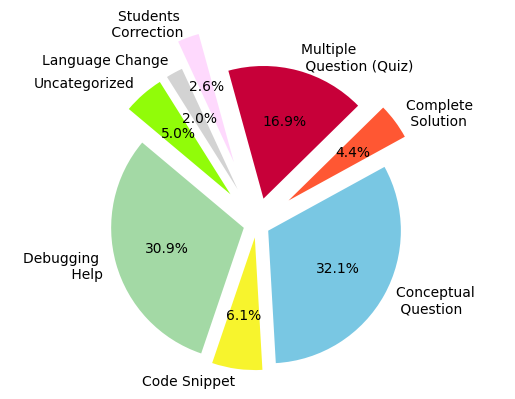
\includegraphics[scale=0.55]{img/figure1.png}
    \caption{Classification of messages.}
    \label{fig:graph1}
\end{figure}

Approximately 64\% of the messages pertain to categories associated with
critical thinking, corroborating with the findings of
\cite{Ghimire24}. In contrast, around 28\% of the messages
indicate a preference among students for ready-made answers.

\section{Conclusion}

The results of this study suggest that students interact with CharlieBot in a
manner that promotes critical thinking. The majority of the messages analyzed
were related to debugging help, conceptual questions, and student correction,
indicating that students are actively engaging with the bot to understand
concepts and solve problems. This is a positive outcome, as it suggests that
CharlieBot is being used as a tool to enhance learning rather than a crutch for
students to rely on.

\section*{ACKNOWLEDGEMENTS}

The authors would like to thank the Federal Institute of Education, Science and
Technology (IFRS) for the partial financial support provided for the execution
of this research.

\bibliographystyle{apalike}
{\small
\bibliography{References}}

\section*{\uppercase{Appendix}}

If any, the appendix should appear directly after the
references without numbering, and not on a new page. To do so please use the
following command: \textit{$\backslash$section*\{APPENDIX\}}

\end{document}

